\documentclass{article}
\usepackage{tikz}
\usepackage{amsmath}
\usepackage{graphicx}
\usepackage{listings}
\usepackage{hyperref}
\usepackage{indentfirst}
\usepackage{color} 
\usepackage[utf8]{inputenc}
\usepackage{amsmath}
\usepackage{mathtools}
\usepackage{blkarray, bigstrut}
\definecolor{mygreen}{RGB}{28,172,0} % color values Red, Green, Blue
\definecolor{mylilas}{RGB}{170,55,241}
\usepackage{listings}
\usepackage{color}

\definecolor{dkgreen}{rgb}{0,0.6,0}
\definecolor{gray}{rgb}{0.5,0.5,0.5}
\definecolor{mauve}{rgb}{0.58,0,0.82}

\lstset{frame=tb,
  language=Octave,
  aboveskip=3mm,
  belowskip=3mm,
  showstringspaces=false,
  columns=flexible,
  basicstyle={\small\ttfamily},
  numbers=none,
  numberstyle=\tiny\color{gray},
  keywordstyle=\color{blue},
  commentstyle=\color{dkgreen},
  stringstyle=\color{mauve},
  breaklines=true,
  breakatwhitespace=true,
  tabsize=3
}


\graphicspath{ {images/} }
\begin{document}
\pagenumbering{gobble} 
\begin{titlepage}
\author{Domen Gašperlin\\Rok Grmek\\Jakob Gaberc Artenjak\\Anže Gregorc\and Matemetično modeliranje, Fakulteta za računalništvo in informatiko}
\title{\textbf{1. Projekt\\Iskanje po zbirki dokumentov}}
\date{April, 2017}

\maketitle
\begin{center}
  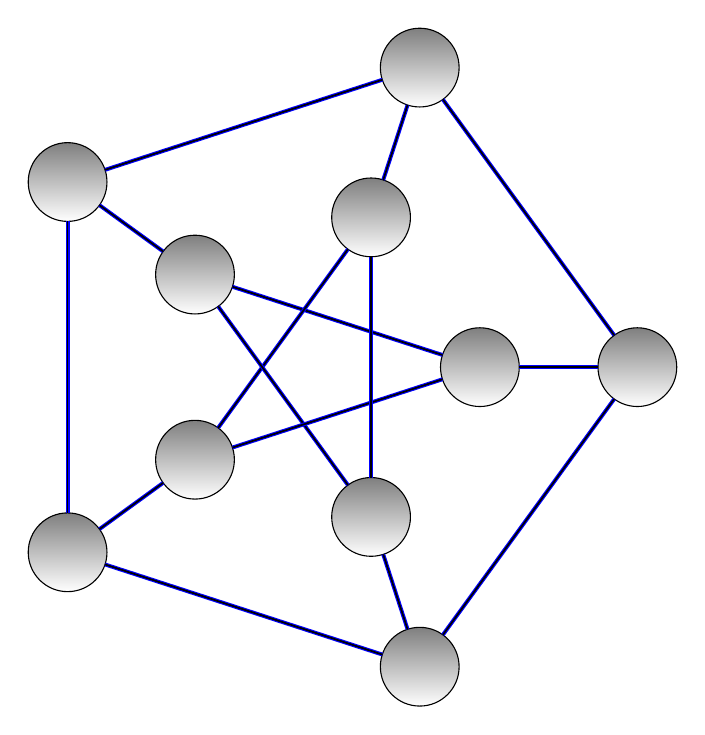
\begin{tikzpicture} 
    \begin{scope} [vertex style/.style={draw,
                                       circle,
                                       minimum size=10mm,
                                       inner sep=0pt,
                                       outer sep=0pt,
                                       shade}] 
      \path \foreach \i in {0,...,4}{%
       (72*\i:2) coordinate[vertex style] (a\i)
       (72*\i:4) coordinate[vertex style] (b\i)}
       ; 
    \end{scope}

     \begin{scope} [edge style/.style={draw=blue,double=black}]
       \foreach \i  in {0,...,4}{%
       \pgfmathtruncatemacro{\nextb}{mod(\i+1,5)}
       \pgfmathtruncatemacro{\nexta}{mod(\i+2,5)} 
       \draw[edge style] (a\i)--(b\i);
       \draw[edge style] (a\i)--(a\nexta);
       \draw[edge style] (b\i)--(b\nextb);
       }  
     \end{scope}

  \end{tikzpicture}
\end{center}
\end{titlepage}

\pagenumbering{arabic}  
\section{Opis problema}
Namen projekta je izdelati iskalnik relevantnih dokumentov po ključnih besedah z metodo\textit{ latentnega semantičnega indeksiranja} (LSI), saj so metode, ki izberejo le dokumente, ki vsebujejo natanko iskane besede, precej nenatačne. Ljudje namreč uporabljamo veliko sopomenk, ki jih preproste metode ne povežejo. Metoda LSI zgradi model, ki združuje več besed v pojme in zato najde tudi dokumente, ki so relevantni, pa ne vsebujejo iskalne besede.

Izdelati je potrebno program, ki bo v dani zbirki za dane ključne besede poiskal najbolj relevantne dokumente.

\section{Naloge}
\subsection{Iz zbirke dokumentov zgradite matriko A povezav med besedami in dokumenti. Vsak dokument naj ima v matriki svoj stolpec, vsaka beseda pa svojo vrstico. Element a\textsubscript{ij} naj bo frekvenca i-te besede v j-tem dokumentu.}

Gradnja matrike A:
\begin{equation*}
  \mathbf{A}=
  \begin{blockarray}{*{5}{c} l}
    \begin{block}{*{5}{>{$\footnotesize}c<{$}} l}
      doc1 & doc2 &  &  docD & \\
    \end{block}
    \begin{block}{[*{5}{c}]>{$\footnotesize}l<{$}}
      a_{11}  & a_{12} & \dots           & a_{1D}       & \bigstrut[t]& beseda1 \\
       a_{11} & a_{12} &                    & \bigstrut[t] &                   &   beseda2 \\
      \vdots   &             & \ddots         &                    &                   &   \vdots  \\
      a_{B1} &              &  \bigstrut[t] & a_{BD}       &                   &  besedaB \\
    \end{block}
  \end{blockarray}
\end{equation*}


\begin{lstlisting}
  f = zeros(length(unique_words), number_of_docs); # matrika f dimenzije (stevilo vseh razlicnih beseded) x (stevilo vseh dokumentov)
  doc_end = 0;
  for i = 1:number_of_docs
    doc_start = doc_end + 1;
    doc_end = doc_start + num_of_words_in_docs(i) - 1;
    f(:, i) = histc(numbers(doc_start:doc_end, 1), all_possible_numbers);
  end
\end{lstlisting}



\end{document}